\documentclass[11pt]{article} % For LaTeX2e

% Change "review" to "final" for the camera-ready version,
% or to "preprint" for a non-anonymous version with page numbers.
\usepackage[review]{acl}

% Standard package includes
\usepackage{times}
\usepackage{latexsym}
\usepackage[T1]{fontenc}
\usepackage[utf8]{inputenc}
\usepackage{microtype}
\usepackage{inconsolata}

\usepackage{booktabs}
\usepackage{multirow}
\usepackage{graphicx}
\usepackage{amsmath}
\usepackage{amssymb}
\usepackage{xcolor}
\usepackage{xspace}

% ---- Custom macros (consistent terminology) ----
\newcommand{\method}{OpenVisTool\xspace}
\newcommand{\dataset}{OpenVisTool-42K\xspace}
\newcommand{\benchname}{OpenVisTool-Bench\xspace}
\newcommand{\toolgain}{tool gain\xspace}
\newcommand{\eg}{e.g.,\xspace}
\newcommand{\ie}{i.e.,\xspace}
\newcommand{\etal}{\textit{et al.}\xspace}
\newcommand{\TODO}[1]{\textcolor{red}{[TODO: #1]}}

\title{\method: An Open Recipe for Synthesizing\\
Cross-Domain Visual Tool-Use Trajectories}

% Author information is hidden under the [review] option for anonymous submission.
\author{Anonymous ACL submission}

\begin{document}

\maketitle

\begin{abstract}
Visual tool-use distillation should teach models how to acquire evidence, not merely how to produce correct final answers. We present \method, a multi-domain trajectory dataset and synthesis recipe for visual tool use. \dataset contains 42K trajectories across Chart, GUI Grounding, Table, Visual Search, and Web-to-HTML tasks, covering complementary visual bottlenecks such as small text, dense layouts, coordinate precision, object search, color or structure analysis, and render-based verification. The key design principle is that a retained trajectory must satisfy two conditions: the task should benefit from tools, and the recorded tool outputs should actually improve solving the task. To enforce this, our pipeline first removes examples that are easily solved without tools, then distills teacher tool-use trajectories, checks final-answer correctness, and filters for \toolgain by measuring whether the teacher's tool observations improve a base model's performance. Fine-tuning on \dataset improves all five domains across four backbones, with average gains of 8.9--13.2 points. Ablations show that correctness and \toolgain filtering are complementary, and comparison with no-tool trajectory SFT shows that tool-use supervision is especially beneficial for evidence-acquisition tasks such as Visual Search and Table.
\end{abstract}

\section{Introduction}
\label{sec:introduction}

Many visual tasks are hard not because the reasoning is abstract, but because the relevant evidence is hard to observe in the original input: reading small axis labels in a chart, aligning a row and column across a low-contrast table, locating a tiny control in a high-resolution screenshot, checking small or occluded objects in a cluttered scene, or rendering generated HTML to verify that its layout matches a reference. In all of these cases the model should actively inspect, transform, mark, or verify the visual input rather than answer from a single static image---the paradigm of \emph{thinking with images} \citep{openai2025o3,su2025thinkingsurvey}, in which a model acts on the visual input as part of its reasoning chain rather than reasoning over a fixed view.

Teaching this behavior through supervised distillation requires trajectories that record the evidence-acquisition process: what the model chose to inspect, what the tool returned, and how the new observation changed its subsequent reasoning. This is exactly where building such data is hard. A dataset that records only final answers misses the process, while one that retains arbitrary tool calls teaches the model to imitate tool-use syntax rather than to use tools when they help. The standard recipe---distill from a strong teacher and keep a trajectory whenever its final answer is correct---does not resolve this tension: a teacher can reach the right answer through unnecessary tool calls, and final-answer correctness reveals neither whether the task needed tools nor whether the recorded observations actually helped.

We therefore argue that a retained trajectory must satisfy two conditions: the task should benefit from tools, and the recorded tool outputs should measurably improve solving it. We operationalize both with \method, an open recipe that curates trajectories by double rejection sampling. We first discard queries a base model already solves without tools, so that external evidence has room to help. We then roll out a strong teacher under a unified visual toolset and keep a trajectory only when it is both \emph{answer-correct}, verified by domain-appropriate evaluators (rule-based matching, an LLM judge, or render-based VLM judging for Web-to-HTML), and \emph{tool-gainful}: prepending the teacher's tool observations to a base model's context must improve its accuracy on the query. The main \dataset is the intersection of the two sets.

The resulting \dataset contains 42K trajectories spanning five domains chosen for complementary visual bottlenecks: Chart and Table stress fine-grained reading and structural alignment, GUI Grounding stresses local inspection and coordinate precision, Visual Search stresses active evidence search in cluttered scenes, and Web-to-HTML stresses a generate-render-observe-revise loop. All domains share one visual toolset---cropping, marking, color and structure analysis, rendering, and final action expression---so the model learns reusable operations rather than a separate interface per task.

Fine-tuning on \dataset improves all five domains across four backbones spanning two model families and 4B--27B scale. On Qwen3.5-9B the average rises from 32.6 to 45.8, with the largest gains where tools expose otherwise-hidden evidence (Visual Search +23.8, Table +17.3). Controlled variants confirm the design: correctness-only and tool-gain-only filtering each underperform their intersection on every domain, and against a no-tool trajectory SFT baseline trained on the same queries, tool-use supervision wins on four of five domains and by 8.7 average points. The exception, GUI Grounding, is instructive rather than hidden: when the metric rewards a single coordinate, direct imitation can be more sample-efficient than a multi-step protocol of cropping, coordinate remapping, and action formatting. Visual tool-use distillation is thus not a uniform replacement for all supervision; its advantage is sharpest when tools acquire new visual evidence.

In summary, our contributions are:
\begin{itemize}
  \item We present \method, an open pipeline for synthesizing multi-domain visual tool-use trajectories under a shared visual toolset.
  \item We construct \dataset, a 42K-example corpus covering Chart, GUI Grounding, Table, Visual Search, and Web-to-HTML, chosen for complementary visual bottlenecks and tool demands.
  \item We propose double rejection sampling based on task difficulty, final-answer correctness, and \toolgain, retaining only trajectories that both solve the task and contain tool observations that improve solvability.
  \item We provide controlled dataset variants and experiments showing that the correctness and \toolgain filters are complementary, that tool-use trajectories outperform no-tool trajectories on evidence-acquisition domains, and that GUI Grounding exposes a useful limitation of the current action protocol.
\end{itemize}

\section{Related Work}
\label{sec:related_work}

% Organize methodologically (by line of work), not paper-by-paper.

\paragraph{Think with Images}
Rather than reasoning over a single static view, a model can make visual operations part of its reasoning chain---the \emph{thinking with images} paradigm popularized by OpenAI o3 \citep{openai2025o3,su2025thinkingsurvey}. Early realizations orchestrate external modules around a frozen model: visual programming composes specialist tools through generated code \citep{gupta2023visprog,suris2023vipergpt}, V$^{*}$ \citep{wu2024vstar} attaches an LLM-guided visual search module for high-resolution images, Visual Sketchpad \citep{hu2024sketchpad} lets the model draw intermediate visual artifacts, and CogCoM \citep{qi2024cogcom} distills a chain of image manipulations into the model itself. A second line uses reinforcement learning to incentivize native interleaved image--text reasoning: DeepEyes \citep{zheng2026deepeyes} elicits emergent crop-and-reexamine behavior from the model's own grounding ability without cold-start SFT, Pixel Reasoner \citep{su2026pixelreasoner} adds curiosity-driven rewards to escape the textual-reasoning shortcut, and OpenThinkIMG \citep{su2025openthinkimg} and Visual-ARFT \citep{liu2025visualarft} optimize policies for invoking external vision tools. Recent systems scale the action space and interaction depth: Thyme \citep{zhang2026theme} executes model-generated code for free-form image operations and numerical computation, Mini-o3 \citep{lai2026minio3} scales trial-and-error visual search to tens of interaction turns, and DeepEyesV2 \citep{hong2026deepeyesv2} unifies image operations, code execution, and web search in a single reasoning loop. Notably, several of these report that RL alone fails to induce robust tool use, making a cold-start SFT stage on curated trajectories indispensable \citep{hong2026deepeyesv2,zhang2026theme,lai2026minio3}. This line of work advances training algorithms and model capability, typically on one or two domains such as high-resolution visual search, while the trajectory corpora that bootstrap these systems remain largely in-house and domain-specific. \method targets the complementary data side: an open, cross-domain recipe for synthesizing visual tool-use trajectories that can serve as cold-start supervision for such models.

\paragraph{Agentic Trajectory Synthesis}
Because expert demonstrations of multi-step tool use are scarce, a growing body of work synthesizes agent trajectories automatically as training supervision. For text-only tool-use data, Toolformer \citep{schick2023toolformer} self-labels API calls by their effect on language-modeling loss, ToolLLM \citep{qin2024toolllm} generates instruction--solution pairs over 16K+ real-world APIs, APIGen \citep{liu2024apigen} verifies function-calling data through staged format, execution, and semantic checks, and FireAct \citep{chen2023fireact} and AgentTuning \citep{zeng2024agenttuning} distill trajectories from stronger teacher agents for SFT. For GUI and web agents, OS-Genesis \citep{sun2025osgenesis} derives task instructions retroactively from interaction-driven exploration and scores trajectories with a reward model, while AgentTrek \citep{xu2025agenttrek} replays web tutorials under a VLM evaluator. Closest to our setting, multimodal pipelines such as TACO \citep{ma2024taco} and MM-Traj \citep{gao2024mmtraj} generate chains of thought and action with a teacher or programs and then filter them, and the cold-start corpora of Thyme and Mini-o3 are constructed analogously \citep{zhang2026theme,lai2026minio3}. Across these pipelines, quality control instantiates outcome-based rejection sampling \citep{zelikman2022star,yuan2023rft}: a trajectory is kept if its format is valid, its calls execute, or its final answer is correct. None of these filters asks whether the recorded tool interactions are actually \emph{useful}---a teacher can answer correctly while its tool calls are decorative, and many tasks need no tools at all. \method closes this gap with double rejection sampling: difficulty filtering discards queries a base model already solves without tools, and the \toolgain filter retains only trajectories whose tool observations measurably improve a base model's accuracy, applied uniformly across five visual domains under a shared toolset.

\section{\method}
\label{sec:method}

\method curates visual tool-use trajectories so that fine-tuning teaches \emph{evidence acquisition} rather than tool-call mimicry. After fixing notation and retention criteria (\S\ref{sec:overview}), we follow the three pipeline stages of Figure~\ref{fig:pipeline}: source data with a difficulty pre-screen (\S\ref{sec:data}), trajectory synthesis under per-domain tool-use patterns (\S\ref{sec:synthesis}), and double rejection sampling on correctness and tool-use gain (\S\ref{sec:filtering}).

% ============================================================================
% FIGURE 1 --- Data-synthesis flowchart (wide, top of Method). This is the single
% main method figure; the tool-use gain schematic (former Fig. 3) is folded in as an inset.
% Left-to-right:
%   (1) Source corpora grouped into the five domains, each tagged with its bottleneck.
%   (2) Difficulty PRE-SCREEN (before synthesis): probe pi0 = Qwen3.5-9B runs k no-tool
%       rollouts; keep only "hard" queries (no-tool avg@k <= 0.5) -- gate C1.
%   (3) Teacher rollout under the SHARED visual toolset, steered by a per-domain pattern;
%       each step emits thinking -> tool call -> observation.
%   (4) DOUBLE REJECTION SAMPLING (after synthesis): correctness check (rule / LLM-judge /
%       render-VLM) AND tool-use gain check -- gate C2. Intersection = OpenVisTool-42K.
% INSET (tool-use gain): two probes of pi0 on the same query -- no-tool avg@k (p0) vs. avg@k
%   given the teacher's OBSERVATIONS as a prefix (p_pre); keep iff g = p_pre - p0 >= delta.
% ============================================================================
\begin{figure*}[t]
\centering
\fbox{\begin{minipage}[c][3.8cm][c]{0.96\textwidth}
\centering\itshape
[Figure~\ref{fig:pipeline} placeholder]\\[2pt]
End-to-end \method pipeline: five-domain source corpora $\rightarrow$ difficulty pre-screen (no-tool avg@$k$ with the probe $\pi_0$, gate~C1) $\rightarrow$ teacher rollout under the shared visual toolset with per-domain tool-use patterns $\rightarrow$ double rejection sampling (answer correctness $\cap$ positive tool-use gain, gate~C2) $\rightarrow$ \dataset. Inset: the tool-use gain test compares $\pi_0$'s no-tool avg@$k$ ($\bar{p}_0$) with its avg@$k$ given the teacher's observations as a prefix ($\bar{p}_{\mathrm{pre}}$); keep iff $g=\bar{p}_{\mathrm{pre}}-\bar{p}_0\ge\delta$.
\end{minipage}}
\caption{Overview of the \method recipe. A difficulty pre-screen (gate~C1) keeps only queries a base solver cannot answer without tools; after synthesis, double rejection sampling keeps a trajectory only if it is both answer-correct and tool-beneficial---its observations measurably improve that solver (gate~C2, shown in the inset). One visual toolset is shared across all five domains.}
\label{fig:pipeline}
\end{figure*}

% \subsection{Overview and Notation}
\subsection{Problem Formulation and Notation}
\label{sec:overview}
A training instance is a query $q=(x,t)$ pairing one or more images $x$ with a text instruction $t$, from a domain $d\in\{\textsc{Chart},\textsc{GUI},\textsc{Table},\textsc{VisualSearch},\textsc{Web2HTML}\}$ with reference answer $a^\star$. Rolling out a tool-using teacher $\mathcal{T}$ yields a \emph{trajectory} $\zeta=(r_1,c_1,o_1,\dots,r_m,c_m,o_m,\hat{a})$ that interleaves reasoning steps $r_i$, tool calls $c_i$, and observations $o_i$, ending in an answer $\hat{a}$. An observation is the new evidence a tool surfaces---a crop, an annotated overlay, a color mask, a rendered screenshot, or a computed value---produced by a shared visual toolset (detailed in \S\ref{sec:synthesis}).

\paragraph{The spurious supervision problem.}
Existing pipelines retain a trajectory whenever $\hat{a}=a^\star$, implicitly assuming that every answer-correct demonstration provides useful supervision. This conflates correctness with utility. A strong teacher can often reach the right answer without relying on its tool observations---via parametric knowledge or low-resolution cues already in the static encoding. The resulting trajectories are answer-correct yet \emph{spurious}: tools are invoked, but the observations do not causally contribute to the outcome. Training on such trajectories teaches correlation (tool calls co-occur with correct answers) rather than causation (tool observations \emph{enable} correct answers).

\paragraph{Instructive trajectories.}
We define a trajectory $\zeta$ as \emph{instructive} for query $q$ iff it satisfies two conditions jointly:
\begin{itemize}
    \item \textbf{(C1) Outcome validity:} $\hat{a}$ matches $a^\star$---the model is not trained on erroneous reasoning.
    \item \textbf{(C2) Causal utility:} the observations $o_{1:m}$ causally contribute to reaching $a^\star$---counterfactually removing them should degrade performance.
\end{itemize}
Together, C1 and C2 shift the retention question from ``did this trajectory produce a correct answer?''\ to ``did the tool observations \emph{cause} the correct answer?''

\paragraph{Operationalization.}
Testing C2 directly on the teacher $\mathcal{T}$ is uninformative: a strong teacher is often correct regardless of observations. We instead use a weaker \emph{probe} $\pi_0$ (Qwen3.5-9B) that is sensitive to evidence gaps. We compare $\pi_0$'s accuracy on $q$ without observations against its accuracy when the teacher's $o_{1:m}$ are prepended to its context; a positive gain certifies that the observations carry otherwise-unavailable evidence. The recipe is teacher-agnostic; $\mathcal{T}$ (Qwen3.5-Plus) performs rollout throughout.

This criterion is realized through three stages. \textbf{Stage~1} (\S\ref{sec:data}) ensures the problem \emph{requires} tools: queries $\pi_0$ already solves are discarded, establishing that an evidence gap exists. \textbf{Stage~2} (\S\ref{sec:synthesis}) ensures tools are used \emph{coherently}: per-domain patterns steer the teacher toward bottleneck-resolving observations. \textbf{Stage~3} (\S\ref{sec:filtering}) verifies C1$\,\cap\,$C2: dual rejection keeps only trajectories that are answer-correct \emph{and} whose observations measurably improve $\pi_0$. To evaluate whether models trained on instructive trajectories genuinely acquire tool-use ability—rather than memorizing domain-specific patterns—we additionally construct OpenVisTool-Bench, an evaluation suite that isolates tool-decisive instances (§4.1).

% We retain only \emph{useful} tool use, via two conditions. (C1) The query should \emph{benefit} from tools---a base solver should not already answer it from a static view---a property of $q$ enforced as a pre-screen \emph{before} synthesis (\S\ref{sec:data}). (C2) The recorded observations should \emph{causally improve} solving it, not merely co-occur with a correct answer---a property of $\zeta$ enforced \emph{after} synthesis (\S\ref{sec:filtering}). Throughout, a fixed probe $\pi_0$ (Qwen3.5-9B) is the reference base solver and a strong teacher $\mathcal{T}$ (Qwen3.5-Plus) does the rollout; the recipe is teacher-agnostic.

% \paragraph{A shared visual toolset.}
% All domains expose the same toolset, so the model learns reusable operations rather than a per-task interface: \emph{geometric transforms} (\texttt{crop}, \texttt{locate\_in\_crop}, \texttt{rotate}/\texttt{flip}), \emph{annotation aids} (\texttt{draw\_bbox}, \texttt{draw\_line}), \emph{readability enhancement} (\texttt{enhance\_contrast}, \texttt{adjust\_brightness}), \emph{color and structure analysis} (\texttt{in\_range\_color}, \texttt{find\_contours}, \texttt{template\_match}), and \emph{computation and action} (\texttt{exec}/\texttt{write\_file}, \texttt{render\_html}, \texttt{computer\_use}). What differs across domains is which operations are canonical and in what order they fire.

% \subsection{Source Data and Difficulty Pre-Screen}
\subsection{Stage 1: Ensuring Tool Necessity}
\label{sec:data}

Causal utility (C2) is only meaningful when an evidence gap exists: if the probe $\pi_0$ already answers $q$ reliably from a static view, any tool observation is redundant---it may correlate with correctness but cannot \emph{cause} it. Stage~1 therefore establishes the causal premise by retaining only queries that exhibit a genuine perception bottleneck, i.e., where the base solver's visual encoding is insufficient and tools have the opportunity to supply otherwise-unavailable evidence.


\paragraph{Source corpora.}
We assemble \method from public corpora, each domain stressing a distinct visual bottleneck: \textsc{Chart} from ChartVerse-SFT~\citep{chartverse}; \textsc{Table} from CoSyn-400K~\citep{cosyn} and TABLET~\citep{tablet}; \textsc{GUI} from OS-Atlas~\citep{osatlas}, AgentNet~\citep{agentnet}, and UGround~\citep{uground}; \textsc{VisualSearch} from Vero-600K~\citep{vero} and DeepEyesV2~\citep{hong2026deepeyesv2}; and \textsc{Web2HTML} from VinciCoder~\citep{vincicoder}. We keep gold answers $a^\star$ and re-purpose the images as queries. For the grounding-heavy domains we further prefer high-resolution images whose target occupies a small fraction of the frame---the regime where a static encoding is weakest and a crop-and-zoom recovers the detail (appendix).


\paragraph{Difficulty pre-screen.}
% We remove queries a base solver already answers without tools. For each $q$ we run $k$ no-tool rollouts with $\pi_0$ (temperature $0.7$, $k{=}4$), scored by a domain-appropriate evaluator $\mathcal{E}_d\in\{0,1\}$ (\S\ref{sec:filtering}):

For each candidate $q$ we run $k$ no-tool rollouts with $\pi_0$ (temperature $0.7$, $k{=}4$), scored by a domain-appropriate evaluator $\mathcal{E}_d\in\{0,1\}$ (\S\ref{sec:filtering}):
\begin{equation}
\bar{p}_0(q)\;=\;\frac{1}{k}\sum_{j=1}^{k}\mathcal{E}_d\!\left(\pi_0(q)^{(j)},\,a^\star\right).
\label{eq:nopt}
\end{equation}
% We keep $q$ only when $\bar{p}_0(q)\le 0.5$ (uniform across domains) and cache $\bar{p}_0(q)$ as the baseline for the tool-use gain test.
We retain $q$ only when $\bar{p}_0(q)\le 0.5$ (uniform across domains), indicating that $\pi_0$ cannot reliably solve it without external evidence. The cached $\bar{p}_0(q)$ simultaneously serves as the no-tool baseline for the causal gain test in Stage~3 (\S\ref{sec:filtering}). The resulting query pool forms the eligible population over which trajectory synthesis and causal verification operate.

% \subsection{Trajectory Synthesis with Per-Domain Patterns}
\subsection{Stage 2: Structured Trajectory Synthesis}
\label{sec:synthesis}

\paragraph{Why domain-guided patterns.}
A naive approach lets the teacher $\mathcal{T}$ use tools freely. In pilot studies, over 70\% of such trajectories are \emph{decorative}---tools are invoked but their observations do not resolve the actual perception bottleneck, yielding high C2 rejection rates and low data efficiency. We instead steer synthesis with \emph{per-domain patterns}: structured operation sequences derived from the principle that each domain's pattern should target its characteristic visual bottleneck with the minimal tool operations that resolve it. For example, \textsc{GUI} queries typically fail because a small widget is indistinguishable at the static encoding resolution; the corresponding pattern therefore prescribes \emph{detect $\to$ crop-and-zoom $\to$ re-read}, directly supplying the missing fine-grained evidence. \TODO{Maybe use a figure to illustrate this?} All five domains and full prompt templates are summarized in Appendix \ref{app:prompts}. All domains share a single toolset---crop, overlay, color-mask, render, and compute---ensuring that cross-domain transfer experiments (\S\ref{sec:cross_domain}) reflect genuine skill generalization rather than differences in tool interfaces.

\paragraph{Synthesis procedure.}
Given a query $q$ that passed Stage~1, we prompt $\mathcal{T}$ with the domain-specific pattern and the shared tool API, requesting a multi-step trajectory $\zeta$. The pattern acts as a soft constraint: it specifies which bottleneck to address and which operations are expected, but allows $\mathcal{T}$ to adapt the number of steps and to skip unnecessary calls. We illustrate with \textsc{GUI}: the teacher first calls \texttt{detect} to localize candidate elements, then \texttt{crop\_zoom} on the highest-confidence region, and finally re-reads the zoomed patch to extract the widget label---each observation progressively narrows the evidence gap identified in Stage~1. Trajectories that deviate entirely from the prescribed pattern (e.g., invoking only \texttt{compute} for a grounding task) are discarded before entering Stage~3, as they are unlikely to pass causal verification.

% A generic ``use tools when helpful'' prompt elicits decorative or missing calls: the teacher may answer correctly while its calls are incidental, or skip the operation a query needs. We instead give each domain a \emph{tool-use pattern}---a short sequence of canonical operations keyed to its visual bottleneck---and steer the teacher to follow it; one canonical trajectory per domain is shown in appendix Figure~\ref{fig:patterns}. \textbf{Chart/Table}: \texttt{crop} the subplot or cell block, \texttt{draw\_line}/\texttt{draw\_bbox} to align a value with its axis tick or a row with its header, \texttt{in\_range\_color} for legends or highlighted cells, \texttt{exec} for arithmetic. \textbf{GUI}: \texttt{crop} a tight window, click in local coordinates, \texttt{locate\_in\_crop} to remap into the $0$--$1000$ space, and end in one \texttt{computer\_use} click. \textbf{Visual Search}: \texttt{crop} and \texttt{draw\_bbox} to verify and track candidates, \texttt{in\_range\_color} for color-defined targets, \texttt{exec} to aggregate counts. \textbf{Web-to-HTML}: \texttt{write\_file} a draft, \texttt{render\_html}, name the discrepancies against the reference, \texttt{edit\_file}, and re-render until they match.

We realize the patterns through an agent loop (up to $30$ tool rounds): a per-domain instruction injected into the teacher's system prompt gives each tool a concrete trigger and asks it to attach a hypothesis to every call and to call only when it reduces ambiguity, suppressing gratuitous use. Each query runs in an isolated workspace with relativized paths, so trajectories carry no host-specific absolute paths; full prompts are in the appendix.

% \subsection{Double Rejection Sampling}

\subsection{Stage 3: Supervision Quality Verification via Dual Rejection}
\label{sec:filtering}
% We formulate effective tool-use supervision as satisfying two necessary conditions:
% the trajectory must (1)~produce a correct answer, and (2)~contain observations that
% \emph{causally} improve the model's reasoning. We apply \emph{dual rejection sampling},
% retaining only trajectories that pass both criteria.

We retain a synthesized trajectory only if it satisfies two criteria jointly: \textbf{C1 (Correctness)}---the final answer $\hat{a}$ matches the ground truth $a^*$; and \textbf{C2 (Causal Utility)}---the tool observations genuinely improve visual reasoning rather than serving as decoration. C1 is operationalized straightforwardly via answer matching (rule-based for Chart, Table, and Visual Search; point-in-box for GUI; LLM-judged for free-form answers; render-based VLM comparison for Web2HTML). The key methodological contribution of this work lies in the operationalization of C2: the \emph{observation injection test}.

\paragraph{Observation injection test.}
The core question C2 asks is: \emph{do the recorded observations carry visual evidence that is itself causally useful?} We answer this through an interventionist design. Given a trajectory with observations $o_{1:m}$, we \emph{inject} only $o_{1:m}$---without the teacher's reasoning or tool calls---into the student-level probe model $\pi_0$'s context and measure its pass rate $\bar{p}_{\text{pre}}(q)$ over $k$ samples:
\begin{equation}
    \bar{p}_{\text{pre}}(q) \;=\; \frac{1}{k}\sum_{j=1}^{k} \mathcal{E}_d\!\left(\pi_0\!\left(q;\,o_{1:m}\right)^{(j)},\; a^*\right).
\end{equation}
The causal effect of the observations is then $g(q) = \bar{p}_{\text{pre}}(q) - \bar{p}_0(q)$, where $\bar{p}_0(q)$ is the baseline from Stage~1 (\S\ref{sec:data}). We retain the trajectory iff $g(q) \ge \delta$ (we set $\delta=0.1$). Two design choices deserve emphasis. First, we inject observations \emph{alone}, excluding the teacher's reasoning chain; this eliminates teacher reasoning as a confound and isolates the informational value of the visual evidence itself. Second, we probe with the student-level model $\pi_0$ rather than the teacher $\mathcal{T}$: because $\mathcal{T}$ is powerful enough to answer most queries regardless of observation quality, it is insensitive to evidence gaps, whereas $\pi_0$ faithfully reflects whether the observations resolve the bottleneck that originally caused failure.

\paragraph{Complementarity of C1 and C2.}
Neither criterion alone suffices for high-quality supervision. C1 without C2 admits trajectories where the teacher arrives at the correct answer \emph{despite} useless tool calls---training on such data teaches the student to invoke tools decoratively. C2 without C1 may retain trajectories whose observations help $\pi_0$ yet whose reasoning chain contains errors---training on them propagates flawed reasoning. Their intersection defines our retention set: a trajectory is kept if and only if it both demonstrates correct behavior \emph{and} its observations are the causal reason that correctness becomes achievable. We term this conjunction \emph{dual rejection sampling}. For ablation purposes we also release \textsc{correctness-only} and \textsc{tool-use-gain-only} variants (\S\ref{sec:ablation_gain}). The final corpus, \textsc{OpenVisTool-42K}, merges per-domain retained trajectories formatted as multi-turn SFT sessions that preserve the teacher's reasoning, each tool call with its arguments, and the returned observations; tool schemas are extracted from the inference-time implementations to ensure train--test consistency.

% The difficulty pre-screen acts on queries before synthesis. We now apply \emph{double rejection sampling} to the synthesized trajectories, keeping the \emph{intersection} of two filters.

% \paragraph{Correctness.}
% A trajectory is retained only if its final answer $\hat{a}$ matches $a^\star$ under $\mathcal{E}_d$, via three backends: rule-based matching (normalized string/number with tolerance for Chart, Table, and Visual Search; point-in-box for GUI), an LLM judge (Qwen3.5-27B) for free-form answers, and a render-based VLM judge for Web-to-HTML (rendered HTML vs.\ reference). Quality rules additionally reject malformed demonstrations---host absolute paths, missing images, or budget exhaustion without an answer.

% \paragraph{Tool-Use Gain.}
% Correctness alone cannot tell whether the tools \emph{mattered}: a teacher can answer correctly while its observations are decorative. We extract the observations $o_{1:m}$ from a correct trajectory, prepend them---without the teacher's reasoning---to $\pi_0$'s context for the same query, and recompute the pass rate
% \begin{equation}
% \bar{p}_{\mathrm{pre}}(q)\;=\;\frac{1}{k}\sum_{j=1}^{k}\mathcal{E}_d\!\left(\pi_0\big(q\,;\,o_{1:m}\big)^{(j)},\,a^\star\right).
% \label{eq:prefix}
% \end{equation}
% We keep the trajectory iff the gain over the cached baseline, $g(q)=\bar{p}_{\mathrm{pre}}(q)-\bar{p}_0(q)$, clears a threshold ($\delta{=}0.1$). Because only the observations are injected, a positive gain certifies the recorded evidence is itself usable---it raised a base model's accuracy on a query it could not reliably solve before---whereas incidental tools give $g\!\approx\!0$ and are discarded (inset, Figure~\ref{fig:pipeline}).

% \paragraph{The retained corpus.}
% The intersection is the main \dataset; for ablation we also release \emph{correctness-only} and \emph{tool-use-gain-only} variants, the filters being complementary---correctness removes invalid demonstrations, while the tool-use gain filter removes causally useless ones (\S\ref{sec:ablation_gain}). Retained sessions become SFT samples that preserve the teacher's reasoning, each tool call with its arguments, and the returned observation, so fine-tuning supervises \emph{when} and \emph{how} to call tools, not just the answer; tool schemas are extracted from the implementations to match the inference-time agent. Merging per-domain selections gives the 42K-trajectory \dataset (per-domain counts in the appendix); we fine-tune students with tools enabled and evaluate the same backbones without tools (\S\ref{sec:experiments}).

\begin{table*}[t]
\centering

% Keep the compact column spacing local to the tabular.
\begingroup
\setlength{\tabcolsep}{3pt}

\begin{tabularx}{\textwidth}{@{}ll*{6}{Y}@{}}

\toprule
\multirow{2}{*}{\textbf{Model}}
& \multirow{2}{*}{\textbf{Setting}}
& \multicolumn{6}{c}{\textbf{OpenVisTool-Bench}}
\\
\cmidrule(lr){3-8}

& & \textbf{Chart}
& \textbf{GUI}
& \textbf{Table}
& \textbf{VisualSearch}
& \textbf{Web2HTML}
& \textbf{AVG} \\
\midrule

\multirow{2}{*}{GPT-5.5}
& w/o tool
& 63.3
& 17.7
& 48.9
& 27.7
& 51.7
& 41.9 \\

& with tool
& \textbf{66.6}
& 24.2
& \textbf{53.9}
& 46.2
& \textbf{54.3}
& \underline{49.0} \\

\addlinespace[1pt]

\multirow{2}{*}{Kimi K2.6}
& w/o tool
& 50.9
& 17.1
& 34.4
& 13.8
& 49.4
& 37.6 \\

& with tool
& \underline{64.3}
& 18.8
& \underline{51.6}
& 49.8
& \underline{53.6}
& 45.9 \\

\midrule
Qwen2.5-VL-7B
& w/o tool
& 18.2
& 5.1
& 21.2
& 28.3
& 23.1
& 19.2 \\

\addlinespace[1pt]

Thyme
& with tool
& 19.8
& 0.0
& 17.9
& 39.2
& 14.3
& 18.2 \\

\addlinespace[1pt]

DeepEyes V2
& with tool
& 20.9
& 1.7
& 20.4
& 31.8
& 2.4
& 15.5 \\

\midrule
\multirow{2}{*}{Qwen3.5-4B}
& w/o tool
& 31.6
& 22.0
& 25.4
& 34.0
& 40.8
& 30.8 \\

& with tool
& 32.5
& 23.5
& 32.3
& 39.6
& 41.6
& 33.9 \\

\quad+\dataset
& with tool
& 43.0\imp{11.4}
& 27.4\imp{5.4}
& 37.3\imp{11.9}
& 56.6\imp{22.6}
& 43.4\imp{2.6}
& 41.5\imp{10.7} \\

\midrule
\multirow{2}{*}{Qwen3-VL-8B-Instruct}
& w/o tool
& 22.1
& 13.0
& 26.7
& 31.8
& 26.5
& 24.0 \\

& with tool
& 20.9
& 12.6
& 24.6
& 30.2
& 28.1
& 23.3 \\

\quad+\dataset
& with tool
& 26.1\imp{4.0}
& 19.7\imp{6.7}
& 35.3\imp{8.6}
& 50.7\imp{18.9}
& 32.9\imp{6.4}
& 32.9\imp{8.9} \\

\midrule
\multirow{2}{*}{Qwen3.5-9B}
& w/o tool
& 34.6
& 27.1
& 29.0
& 35.6
& 40.1
& 33.3 \\

& with tool
& 28.4
& 24.8
& 26.8
& 38.7
& 42.0
& 32.1 \\

\quad+\dataset
& with tool
& 49.3\imp{14.7}
& \textbf{31.6}\imp{4.5}
& 43.1\imp{14.1}
& \textbf{59.4}\imp{23.8}
& 45.5\imp{5.4}
& 45.8\imp{12.5} \\

\midrule
\multirow{2}{*}{Qwen3.5-27B}
& w/o tool
& 45.7
& 28.9
& 29.8
& 43.2
& 46.6
& 38.8 \\

& with tool
& 47.7
& \underline{29.1}
& 43.3
& 54.7
& 44.3
& 43.8 \\

\quad+\dataset
& with tool
& 60.7\imp{15.0}
& \textbf{31.6}\imp{2.7}
& 48.2\imp{18.4}
& \underline{57.3}\imp{14.1}
& 48.7\imp{2.1}
& \textbf{49.3}\imp{10.5} \\

\bottomrule
\end{tabularx}
\endgroup

\caption{
Main results on OpenVisTool-Bench. Qwen2.5-VL-7B-Instruct is the shared backbone of Thyme and DeepEyes V2. +OpenVisTool-42K rows use our training data, and green $+x$ suffixes show absolute gains over the no-tool baseline. Our data improves the five-domain average by 8.9--12.5 points. \textbf{Bold} and \underline{underlined} entries mark the best and second-best results.
}
\label{tab:main}

\end{table*}


\section{Experiments}
\label{sec:experiments}

We design experiments to validate our central claim—that effective visual tool use is learned from instructive trajectories rather than merely successful ones—and to answer the following questions:
\begin{itemize}
    \item \textbf{Effectiveness:} Does fine-tuning on OpenVisTool-42K teach models to effectively leverage visual tools, and can it lift open-source models to closed-source performance levels? (\S\ref{sec:main_results})
    
    \item \textbf{Generalization:} Does the learned tool-use capability transfer to out-of-distribution visual tasks unseen during training, rather than overfitting to domain-specific tool-calling patterns? (\S\ref{sec:ood})
    
    \item \textbf{Supervision verification:} Are outcome validity and causal utility both necessary for constructing effective visual tool-use supervision? (\S\ref{sec:ablation_gain})
    
    \item \textbf{Cross-domain synergy:} Does visual tool use emerge as a transferable meta-skill across domains, and does multi-domain training resolve strategy conflicts that single-domain training introduces? (\S\ref{sec:cross_domain})
\end{itemize}

\subsection{\benchname: Isolating Tool-Use Ability}
\label{sec:bench}

% We introduce \benchname, a multi-domain evaluation suite specifically designed to measure how effectively models leverage visual tools.
% Unlike existing benchmarks that conflate general visual understanding with tool-augmented reasoning, \benchname{} isolates the incremental value of active tool use by retaining only instances where tools are beneficial.
General-purpose visual benchmarks often mix tool-relevant instances with questions that can already be solved reliably from the initial image encoding. To isolate the incremental value of active tool use, we introduce \benchname, a multi-domain evaluation suite specifically designed to measure how effectively models leverage visual tools.

\paragraph{Design goal.}

\benchname targets tasks that demand active visual evidence acquisition: the information needed to answer correctly is difficult to obtain from a single static view, requiring models to interact with the visual environment (e.g., cropping into regions of interest, enhancing contrast for faint details, or detecting edges and contours to isolate structure) to gather sufficient evidence. Concretely, we retain only the instances for which tool use is clearly beneficial, rather than uniformly sampling from the source benchmarks.


\paragraph{Per-domain construction.}

The two mechanisms below differ in \emph{how} our goal is operationalized, depending on whether the source benchmark already isolates tool-demanding tasks or requires explicit filtering.

\begin{itemize}

\item \textbf{Chart and Table} --- source QA pools are dominated by tool-irrelevant questions, so we \emph{explicitly filter} for tool-decisive instances.
Concretely, we run three strong closed-source models (GPT-5.4, Gemini-3.0-Flash, Qwen3.5-Plus) on every instance under two conditions (with and without tools), each sampled five times.
An instance is retained if, for \emph{any} of the three models, the accuracy gain (avg@5\textsubscript{tool} $-$ avg@5\textsubscript{no-tool}) exceeds a threshold of 0.3, indicating that tool use provides a clear and consistent advantage.
Taking the \emph{union} across models ensures the criterion captures ``tools \emph{in principle} help'' (model-agnostic) rather than ``\emph{our} toolset helps a specific model,'' avoiding circularity with the evaluated students.
We further report results on the complete (unfiltered) Chart and Table source benchmarks in Appendix~\ref{app:fullset}; the consistent gains confirm that our filtering sharpens an existing signal rather than manufactures one.


\item \textbf{GUI, Visual Search, Web-to-HTML} --- unlike the chart/table sources, these benchmarks are \emph{already} curated around a specific visual operation (precise click localization, fine-grained visual retrieval, and faithful layout reproduction, respectively). The tasks inherently require active manipulation of the visual input, making an additional tool-gain filter unnecessary. We therefore adopt them directly: the smallest-target subset of ScreenSpot-Pro (117 items), VisualProbe-Hard, and Vision2Web-Level1.

\end{itemize}


\paragraph{Evaluation protocol.}
Each domain uses an evaluator matched to its task type.
\textbf{Chart, Table, and Visual Search}: an extraction pipeline followed by majority-vote LLM judging yields a binary ($0/1$) correctness score.
\textbf{GUI}: a prediction is correct if the predicted click coordinate falls within the ground-truth bounding box.
\textbf{Web-to-HTML}: we render the generated HTML and compute component-level visual fidelity against the reference page (scaled $0$--$100$).
We report per-domain scores and their macro-average under the avg@$k$ protocol.


\subsection{Experimental Setup}
\label{sec:setup}

\paragraph{Benchmarks.}
We primarily evaluate on \benchname, which covers diverse visual tool-use scenarios across multiple domains. To assess generalization, we additionally test on Agentic-MME and VTC-Bench. We also report results on the full Chart and Table source benchmarks to confirm that gains are not artifacts of our data filtering (Appendix~\ref{app:fullset}).

\paragraph{Baselines.}
We compare three types of models. (i)~General-purpose frontier models: GPT-5.5 and Kimi K2.6~\citep{kimik26blog}, both evaluated without tools and with our shared toolset. (ii)~Smaller-scale general-purpose models: Qwen2.5-VL-7B~\citep{Qwen2.5-VL}, Qwen3-VL-8B-Instruct~\citep{Qwen3-VL} and Qwen3.5~\citep{qwen35blog} series are evaluated both without tools and with our shared toolset before fine-tuning. (iii)~Open-source visual tool-use agents: Thyme~\citep{zhang2026thyme} and DeepEyes V2~\citep{hong2026deepeyesv2}, evaluated with the code-based tool environments used in their original work rather than our toolset.

\paragraph{Training.}
We fine-tune four base models: Qwen3.5-4B/9B/27B and Qwen3-VL-8B-Instruct. All models are trained on \dataset for 3 epochs using SWIFT~\citep{zhao2025swift}. More implementation details are provided in Appendix \ref{app:implement}.

\subsection{Main Results}
\label{sec:main_results}
Table~\ref{tab:main} summarizes performance across all models. We highlight several key findings below.

\paragraph{Consistent gains across all base models and domains.}
Our method yields substantial improvements over the no-tool baselines across all domains and model scales. Across models ranging from 4B to 27B, fine-tuning with \dataset{} brings an average gain of 10.7 points on \benchname, with the most pronounced improvement observed in VisualSearch (+23.8 points). 
Notably, even without any fine-tuning, simply equipping strong off-the-shelf models with our toolset provides significant benefits: the closed-source GPT-5.5 and the open-source Kimi K2.6 achieve 7.1 and 14.1 absolute gains, respectively, demonstrating the inherent utility of the designed tools.
However, for smaller open-source models, naively providing tools without dedicated training yields marginal or even negative returns—Qwen3.5-9B, for instance. After fine-tuning on \dataset, these same models learn to leverage tools effectively, comparable to closed-source models. For example, Qwen3.5-9B with our training achieves an average of 45.8, surpassing GPT-5.5's 41.9 without tools and closely approaching its tool-augmented performance of 49.0.
In contrast, existing tool-use models Thyme and DeepEyes V2, trained on narrow single-domain data, perform worse on the five-domain average than vanilla base models \emph{without any tool access}—they improve on their specialty but collapse catastrophically elsewhere. This comparison highlights that a diverse, multi-domain training corpus, as provided by \dataset{}, is essential for robust and generalizable visual tool use.

\paragraph{Largest gains emerge where tools unlock new visual evidence.}
For domains where the answer is largely derivable from surface-level visual content—such as Chart, which primarily tests text and semantic extraction from images—a sufficiently capable model can already perform well without tools (e.g., GPT-5.5 scores 63.3 on Chart without tools). However, for more challenging domains involving dense details and hidden evidence—such as VisualSearch, which demands fine-grained spatial and geometric reasoning—models often struggle to succeed with their inherent visual perception alone. In these scenarios, invoking auxiliary tools to crop, zoom, or reformat visual content becomes essential. This explains why our method yields the most substantial gains precisely in these demanding domains (e.g., Qwen3.5-9B: +23.8 points on VisualSearch), where tools effectively bridge the gap between what the model can perceive and what the task requires.


\subsection{Out-of-Distribution Generalization}
\label{sec:ood}

\begin{table}[t]
\centering

\begingroup
\small
\setlength{\tabcolsep}{4pt}
\begin{tabular*}{\columnwidth}{@{\extracolsep{\fill}}lcc@{}}

\toprule
\textbf{Model}
& \textbf{Agentic-MME}
& \textbf{VTC-Bench} \\
\midrule

Qwen3.5-4B
& 29.9
& 27.5 \\

\quad+\dataset
& 34.5\imp{4.6}
& 38.8\imp{11.3} \\

\midrule
Qwen3-VL-8B-Instruct
& 25.6
& 28.2 \\

\quad+\dataset
& 32.3\imp{6.7}
& 29.1\imp{0.9} \\

\midrule
Qwen3.5-9B
& 32.7
& 30.1 \\

\quad+\dataset
& \textbf{41.6}\imp{8.9}
& \underline{41.4}\imp{11.3} \\

\midrule
Qwen3.5-27B
& 37.1
& 34.9 \\

\quad+\dataset
& \underline{41.1}\imp{4.0}
& \textbf{45.2}\imp{10.3} \\

\bottomrule
\end{tabular*}
\endgroup

\caption{
Out-of-distribution results on Agentic-MME and VTC-Bench. Untrained backbones are evaluated without tools, while +OpenVisTool-42K models are evaluated with tools. Green $+x$ suffixes show absolute gains over the corresponding no-tool backbone. \textbf{Bold} and \underline{underlined} entries mark the best and second-best results.
}
\label{tab:ood}

\end{table}


To test whether the tool-use capability learned from our five training domains transfers beyond them, we further evaluate on Agentic-MME and VTC-Bench with out-of-distribution domains held out from training. Table~\ref{tab:ood} directly compares each off-the-shelf backbone with its \dataset-trained counterpart, with tools enabled for every model. Training improves all four backbones on both benchmarks, by 1.3--7.9 points on Agentic-MME and 3.9--17.6 points on VTC-Bench. Notably, Qwen3.5-9B rises from 23.8 to 41.4 on VTC-Bench after training. These gains indicate that \dataset teaches a transferable tool-use policy rather than a domain-specific invocation pattern.

\begin{figure}[t]
    \centering
    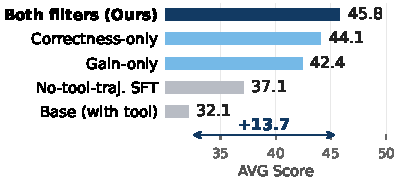
\includegraphics[width=0.9\columnwidth]{figures/fig_ablation.pdf}
    % \caption{Comparison of training variants.}
    \caption{Ablation of the criteria for instructive tool-use supervision on Qwen3.5-9B under a fixed training budget. Requiring both outcome validity and causal utility achieves the best performance, outperforming either criterion alone and the no-tool-trajectory SFT baseline.}
    \label{fig:ablation}
\end{figure}

\begin{table}[t]
    \centering
    \small
    \setlength{\tabcolsep}{3.5pt}
    \begin{tabular}{@{}lccc@{}}
    \toprule
    \textbf{Trajectory source} & \textbf{\shortstack{OpenVisTool-\\Bench}} & \textbf{\shortstack{Agentic-\\MME}} & \textbf{\shortstack{VTC-\\Bench}} \\
    \midrule
    None (Qwen3.5-9B w/o tool) & 33.3 & 32.7 & 30.1 \\
    Correctness-only model & 42.1 & 36.5 & 36.5 \\
    Instructive model (ours) & \textbf{44.5} & \textbf{37.7} & \textbf{38.1} \\
    \bottomrule
    \end{tabular}
    \caption{Trajectory replay analysis using the original Qwen3.5-9B probe model. The probe model answers each query conditioned on the tool call arguments and returned observations generated by the correctness-only or instructively trained model. The generator's reasoning and final answer are excluded. ``None'' denotes evaluation without tool access or trajectory replay.}
    \label{tab:trajectory_replay}
\end{table}


\subsection{Ablation Study}
\label{sec:ablation_gain}
\label{sec:notool_traj}
To validate that effective visual tool-use learning requires both correct answers and causally useful tool traces, we compare four Qwen3.5-9B supervision variants under the same training budget. The first three use tool trajectories retained by (1)~both outcome validity and causal utility (full \dataset{}), (2)~outcome validity alone, or (3)~causal utility alone. The fourth is a no-tool-trajectory SFT baseline, constructed by re-synthesizing trajectories without tool invocation for the queries in the full variant.


\paragraph{Gains originate from tool-use, not from SFT alone.}
As shown in Figure~\ref{fig:ablation}, every tool-augmented variant outperforms the no-tool-trajectory SFT baseline, confirming that improvements stem from learned tool invocation rather than simply training on additional difficult queries.


\paragraph{Both filters are complementary and necessary.}
Intersecting both filters consistently dominates either filter in isolation, with outcome-validity-only and causal-utility-only trailing by 1.7 and 3.4 points, respectively.
The two filters address distinct failure modes: outcome validity removes demonstrations that lead to incorrect answers and would teach erroneous behavior, while causal utility discards trajectories where tools are invoked but their observations contribute no measurable benefit to reaching the solution. Their combination yields the highest-quality training signal.


\paragraph{Instructive filtering yields more useful tool interactions.}
To probe the learned behavior beyond the accuracy of the fine-tuned models themselves, we replay their tool-interaction trajectories to the original Qwen3.5-9B probe model. The replayed context contains only tool call arguments and returned observations; all reasoning and final answers from the trajectory-generating model are excluded, ruling out direct copying of the generator's answer or imitation of its rationale. As shown in Table~\ref{tab:trajectory_replay}, trajectories from both trained models improve the base model on all three benchmarks, but those from the instructively trained model consistently outperform correctness-only trajectories. This behavior-level transfer suggests that causal-utility filtering induces an evidence-acquisition policy whose resulting interactions are more useful to another model, rather than merely producing tool calls that accompany successful outcomes.

\begin{table*}[t]
\centering
\small

\begin{tabular}{llcccccc}
\toprule
\textbf{Variant} & \textbf{Setting} & \textbf{Chart} & \textbf{GUI} & \textbf{Table} & \textbf{VisualSearch} & \textbf{Web2HTML} & \textbf{AVG} \\
\midrule
\multirow{2}{*}{Qwen3.5-9B} & w/o tool & 34.6 & 27.1 & 29.0 & 35.6 & 40.1 & 33.3 \\
 & with tool & 28.4 & 24.8 & 26.8 & 38.7 & 42.0 & 32.1 \\
\midrule
+ \dataset{} (full) & with tool & \textbf{49.3} & \underline{31.6} & \textbf{43.1} & \textbf{59.4} & \textbf{45.5} & \textbf{45.8} \\
\midrule
\multicolumn{8}{l}{\textit{Single-domain slices}} \\
\quad + Chart & with tool & \underline{46.6} & 22.2 & 37.1 & 44.3 & 36.5 & 37.4 \\
\quad + GUI & with tool & 41.4 & \textbf{36.3} & 38.7 & 52.8 & 39.1 & \underline{41.7} \\
\quad + Table & with tool & 45.7 & 20.5 & \underline{38.9} & 45.8 & 39.2 & 38.0 \\
\quad + VisualSearch & with tool & 45.7 & 23.3 & 40.9 & \underline{57.3} & 21.6 & 37.8 \\
\quad + Web2HTML & with tool & 41.6 & 18.2 & 38.5 & 42.2 & \underline{44.6} & 37.0 \\
\bottomrule
\end{tabular}

\caption{Cross-domain transfer with Qwen3.5-9B. We fine-tune the model on either the full \dataset{} mixture or an individual domain slice and evaluate all fine-tuned variants with tools across the five domains.}
\label{tab:cross}

\end{table*}


\subsection{Cross-Domain Transfer}
\label{sec:cross_domain}

% \paragraph{Setup.}
We fine-tune Qwen3.5-9B on each single-domain slice of \dataset{} separately and evaluate on all five domains. Full results are reported in Table~\ref{tab:cross}.

\paragraph{Tool-use transfers as a domain-general meta-skill.}
Training on any single domain improves overall performance over the tool-enabled base model, with gains often extending to domains unseen during training. Most notably, GUI-only training improves VisualSearch by 14.1 points. This cross-domain benefit suggests that the model learns reusable tool-use primitives, such as localized cropping and spatial grounding, rather than only domain-specific solutions.

\paragraph{Transfer is asymmetric, with both positive and negative effects.}
The transfer is not uniformly beneficial because different domains reward different interaction patterns. For example, VisualSearch-only training lowers Web2HTML performance from 42.0 to 21.6. We attribute this degradation to a mismatch in tool-use strategies: repeatedly cropping small regions is effective for fine-grained search but conflicts with the global, full-page reasoning. Single-domain training can therefore over-specialize the tool-use policy and harm domains that require incompatible strategies.

\paragraph{The full mixture resolves strategy conflicts.}
The full \dataset{} mixture achieves a 45.8 average, surpassing all single-domain variants, and performs best on four of the five domains. Exposure to diverse interaction patterns helps the model resolve strategy conflicts through \emph{context-conditional} tool use: it learns not only how to invoke tools, but also which strategy is appropriate for the visual input.

\paragraph{The GUI exception.}
GUI is the only domain where a specialist trained on its single-domain slice outperforms the full mixture on the corresponding domain. A likely reason is that the point-in-bbox metric rewards a single precise click, making direct imitation especially effective, whereas other domains emphasize multi-step interactions such as crop$\to$OCR. Because the full mixture still improves GUI over the untuned tool-enabled base model, this exception points to domain-adaptive mixture weighting rather than a failure of multi-domain tool-use supervision.

\section{Discussion}
\label{sec:analysis}

\subsection{Cross-Domain Transfer}
\label{sec:cross_domain}

To understand whether visual tool-use behavior transfers across domains, we fine-tune Qwen3.5-9B on each single-domain slice of \dataset and evaluate each model on all five domains. Table~\ref{tab:cross} shows that single-domain training often improves out-of-domain performance, but the transfer is highly asymmetric. For example, GUI-only training raises Visual Search from 35.6 to 52.8, and Visual-Search-only training raises Table from 25.8 to 40.9. These gains suggest that some behaviors, such as inspecting localized image regions and grounding visual evidence before answering, are reusable across domains.

At the same time, no single domain is a substitute for the full corpus. \dataset obtains the best average score, and it is best on four of the five evaluation domains. GUI is the exception: the GUI-only slice reaches 36.3, while the full corpus reaches 31.6. This mirrors the no-tool trajectory result in Table~\ref{tab:notool} and indicates that GUI Grounding is unusually sensitive to the training mixture and action format.

\begin{table*}[t]
\centering
\small
\setlength{\tabcolsep}{5pt}
\begin{tabular}{lrrrrrr}
\toprule
Train slice (Qwen3.5-9B) & Chart & GUI & Table & Vis.\ Search & Web2HTML & AVG \\
\midrule
w/o tool          & 34.6 & 27.1 & 25.8 & 35.6 & 40.1 & 32.6 \\
\midrule
Chart             & 46.6 & 22.2 & 37.1 & 44.3 & 36.5 & 37.4 \\
GUI               & 41.4 & \textbf{36.3} & 38.7 & 52.8 & 39.1 & 41.7 \\
Table             & 45.7 & 20.5 & 38.9 & 45.8 & 39.2 & 38.0 \\
Visual Search     & 45.7 & 23.3 & 40.9 & 57.3 & 21.6 & 37.8 \\
Web2HTML          & 41.6 & 18.2 & 38.5 & 42.2 & 44.6 & 37.0 \\
\midrule
\dataset          & \textbf{49.3} & 31.6 & \textbf{43.1} & \textbf{59.4} & \textbf{45.5} & \textbf{45.8} \\
\bottomrule
\end{tabular}
\caption{Cross-domain transfer. Each single-domain row trains on one slice of \dataset for three epochs and evaluates on all domains. Bold marks the best score in each evaluation column. The full \dataset row is shown for reference.}
\label{tab:cross}
\end{table*}

\subsection{Interpreting the GUI Exception}
\label{sec:gui_exception}

GUI Grounding is the only domain where text-only trajectory SFT is stronger than OpenVisTool tool-use SFT: 40.0 versus 31.6. We report this directly because it clarifies what the current recipe does and does not solve. The result does not mean that tool-use supervision is useless for GUI: \dataset still improves the raw Qwen3.5-9B baseline from 27.1 to 31.6, and the GUI-only tool-use slice reaches 36.3. Rather, the result suggests that our current GUI tool protocol is less sample-efficient than direct point imitation under a point-in-box metric.

There are two likely causes. First, GUI Grounding has a very narrow output space: the model ultimately needs to emit one coordinate. A no-tool trajectory can train this behavior directly, whereas a tool-use trajectory introduces extra decisions such as where to crop, how to map crop-local evidence back to the original screenshot, and when to issue the final \texttt{computer\_use} action. Second, cross-domain training appears to dilute GUI-specific action patterns. Most non-GUI single-domain slices reduce GUI performance below the raw baseline, and the GUI-only slice outperforms the full mixture on GUI. This points to GUI-specific interface design and mixture balancing as important future improvements.

\subsection{What the Filtering Ablation Shows}
\label{sec:filtering_discussion}

The filtering ablation supports the central data-quality claim. Correctness alone produces a strong corpus, but it can retain trajectories where the final answer is right even if the tool calls are incidental. Tool-gain filtering addresses that failure mode, and adding it to the correctness filter improves every domain despite reducing the corpus to 42K examples. Conversely, tool-gain-only is weaker than correctness-only, showing that a useful-looking tool prefix is not enough if the teacher trajectory itself is unreliable.

The effect is largest on Table and Visual Search. Compared with correctness-only, the full \dataset gains +4.2 on Table and +2.1 on Visual Search; compared with tool-gain-only, it gains +5.6 and +4.7. These are the domains where the model most needs to acquire evidence through tool outputs, so they benefit most from retaining trajectories that are both correct and causally useful.

\subsection{Takeaway}
\label{sec:analysis_takeaway}

The results support a nuanced view of visual tool-use distillation. Tool-use trajectories are most valuable for evidence-acquisition tasks, where the tool output reveals information that the model cannot reliably infer from the original input. This explains the large gains on Visual Search, Table, and Chart, as well as the advantage over no-tool trajectory SFT on four of five domains. GUI Grounding exposes a limitation: when the benchmark rewards a single precise action, direct imitation can outperform the current multi-step tool-use protocol. We therefore frame OpenVisTool as a strong cross-domain recipe for visual tool-use data, while treating GUI as a diagnostic case for better action interfaces and domain-aware mixing.

\section{Conclusion}
\label{sec:conclusion}
In this work, we introduce \method, a framework for constructing \textbf{instructive} visual tool-use trajectories that addresses a limitation of outcome-only filtering: an answer-correct trajectory may contain tool observations that do not contribute to its answer. \method defines instructive supervision through outcome validity and causal utility, and operationalizes these criteria with difficulty screening, domain-specific tool-use patterns, and supervision verification to construct \dataset across five domains. We separately build \benchname across the same domains to evaluate models' ability to acquire and use visual evidence through tools. Across four backbones, training on \dataset consistently improves performance. Trajectory replay and cross-domain results further suggest that instructive supervision promotes useful evidence acquisition and transferable tool-use behavior.


\section*{Limitations}
% Honest limitations -- reviewers are instructed not to penalize honesty.
\TODO{Candidate limitations to discuss:}
\begin{itemize}
  \item The \toolgain metric is estimated with a specific base model and $k$;
  the threshold $\tau$ is a hyperparameter and the gain estimate is noisy at
  small $k$.
  \item Trajectories are distilled from a single teacher; quality and tool-use
  style are bounded by the teacher's behavior.
  \item Coverage is five domains and one toolset; other visual tools and
  domains are out of scope.
  \item SFT only; we do not study RL or test-time tool-use scaling.
  \item Answer-correctness backends (rule / judge / render) have their own
  error rates that propagate into the retained set.
\end{itemize}


\section*{Ethics Statement}
% Optional but encouraged.
\TODO{Note source-dataset licenses and that released data inherits them;
any image-content / PII considerations for GUI screenshots and web pages;
intended use of the released dataset and pipeline.}


\bibliography{custom}

\appendix
\section{Appendix}
\label{sec:appendix}

\subsection{Pipeline Configuration Details}
\label{app:pipeline}

\paragraph{Teacher rollout.}
Trajectories are synthesized by running the teacher $\mathcal{T}$ (Qwen3.5-Plus) as a tool-using agent in an agent loop: at each turn the teacher emits a reasoning step and an optional tool call, the tool executes in a per-query sandbox, and the resulting observation is appended to the context for the next turn. The loop terminates when the teacher emits a final answer or, for GUI Grounding, the terminal \texttt{computer\_use} click; it is capped at $30$ tool rounds. The recipe is teacher-agnostic and we also support Gemini as an alternative teacher. Rollout is parallelized across queries with a configurable worker pool, and recoverable API errors are retried so that long batches resume cleanly.

\paragraph{Per-query isolation and path safety.}
Each query runs in its own workspace with a private media directory, so the files a tool produces (crops, annotated overlays, color masks, rendered screenshots) never collide across queries. All paths written into a trajectory are relativized to that workspace, so the exported SFT samples contain no host-specific absolute paths; trajectories that nonetheless reference an absolute host path or a missing image are dropped by the correctness stage (\S\ref{sec:filtering}).

\paragraph{Per-domain instructions.}
The tool-use pattern for each domain is supplied as a domain-specific instruction injected into the teacher's system prompt at rollout time, on top of the shared toolset. These instructions enumerate, per tool, a concrete trigger tied to the domain's visual bottleneck, and---for GUI Grounding and Web-to-HTML---prescribe a required multi-step workflow (\S\ref{app:prompts}).

\paragraph{Conversion to SFT.}
Retained sessions are converted to ms-swift training samples that preserve the teacher's reasoning, every tool call with its arguments, and each returned observation. Tool JSON schemas are extracted automatically from the toolset implementations rather than maintained by hand, so the supervised interface matches the agent the student runs at inference.

\subsection{Difficulty and Tool-Gain Hyperparameters}
\label{app:hyperparams}

Table~\ref{tab:hparams} lists the hyperparameters of the three measurement stages. Both the difficulty filter and the \toolgain probe use the same fixed base model $\pi_0$ (Qwen3.5-9B), so the two pass rates $\bar{p}_0$ and $\bar{p}_{\mathrm{pre}}$ are directly comparable when forming the gain $g=\bar{p}_{\mathrm{pre}}-\bar{p}_0$. Difficulty filtering keeps a query when its no-tool avg@$k$ is at most $0.5$, uniformly across domains; the \toolgain filter keeps a trajectory when $g\ge 0.1$. The per-domain answer evaluator $\mathcal{E}_d$ is shared by all stages: rule-based matching for Chart, Table, and Visual Search (point-in-box for GUI), an LLM judge (Qwen3.5-27B) where surface matching is brittle, and a render-based VLM judge for Web-to-HTML.

\begin{table}[t]
\centering
\small
\setlength{\tabcolsep}{4pt}
\begin{tabular}{lll}
\toprule
 & Difficulty filter & \toolgain probe \\
\midrule
Probe model $\pi_0$ & Qwen3.5-9B & Qwen3.5-9B \\
Rollouts $k$ (avg@$k$) & 4 & 4 \\
Temperature & 0.7 & 0.7 \\
Max new tokens & 32768 & 16384 \\
Observation prefix & --- & teacher $o_{1:m}$ \\
Per-obs.\ char limit & --- & 10000 \\
Keep rule & $\bar{p}_0(q)\le 0.5$ & $g(q)\ge 0.1$ \\
\bottomrule
\end{tabular}
\caption{Hyperparameters for difficulty filtering and \toolgain probing. Both stages share the base model $\pi_0$ and the per-domain evaluator $\mathcal{E}_d$. Answer judging uses Qwen3.5-27B; the teacher used for rollout is Qwen3.5-Plus.}
\label{tab:hparams}
\end{table}

\subsection{Dataset Card}
\label{app:datacard}

\paragraph{Sources and selection.}
Table~\ref{tab:datacard} maps each domain to its source corpora, the pre-rollout selection applied, and the answer-evaluation backend. The grounding-heavy domains (GUI, Visual Search) are pre-filtered to high-resolution images with small targets, the regime where a single static encoding is weakest; every domain is then difficulty-filtered to no-tool avg@$k\le 0.5$ before teacher rollout.

\paragraph{Released variants.}
We release three corpora built from the same trajectories under different retention rules: \texttt{OpenVisTool} (the main \dataset, correctness~$\cap$~\toolgain), \texttt{OpenVisTool\_acc\_only} (correctness only), and \texttt{OpenVisTool\_toolgain\_only} (\toolgain only). We additionally provide a no-tool counterpart on the same queries for the trajectory-format ablation of \S\ref{sec:notool_traj}. Per-domain sample counts before and after each filter stage, source licenses, and split sizes are released with the dataset. \TODO{Fill per-domain counts before/after difficulty, correctness, and \toolgain filtering, and source licenses.}

\begin{table}[t]
\centering
\small
\setlength{\tabcolsep}{3pt}
\begin{tabular}{llll}
\toprule
Domain & Source corpora & Pre-selection & Eval \\
\midrule
Chart & ChartVerse-SFT & avg@$k\le0.5$ & rule \\
Table & CoSyn-400K, TABLET & avg@$k\le0.5$ & judge \\
GUI & OS-Atlas, AgentNet, & high-res, & point- \\
 & \;UGround & \;small bbox & \;in-box \\
Vis.\ Search & Vero-600K, DeepEyesV2 & high-res scenes & rule \\
Web2HTML & VinciCoder & avg@$k\le0.5$ & render-VLM \\
\bottomrule
\end{tabular}
\caption{Dataset card. Each domain's source corpora, the pre-rollout selection (all domains additionally pass the uniform no-tool avg@$k\le0.5$ difficulty filter), and the answer-evaluation backend used by the correctness filter.}
\label{tab:datacard}
\end{table}

\subsection{Qualitative Trajectory Examples}
\label{app:qualitative}

\TODO{Rendered thinking~+~tool-call~+~tool-output trajectories, one or two per domain: a Chart \texttt{crop}+\texttt{draw\_line} read, a GUI \texttt{crop}$\to$\texttt{locate\_in\_crop}$\to$\texttt{computer\_use} click, a Visual Search \texttt{crop}+\texttt{draw\_bbox} verification, and a Web-to-HTML \texttt{render\_html}$\to$\texttt{edit\_file} revision loop. Pair each with its $\bar{p}_0$, $\bar{p}_{\mathrm{pre}}$, and gain $g$ to illustrate the \toolgain criterion.}

\subsection{Prompts}
\label{app:prompts}

\paragraph{System prompt.}
The teacher's system prompt is assembled dynamically from the enabled toolset: the tool schemas in effect for a run are inserted automatically, and the per-domain instruction is appended on top. Because the same assembly is used at inference, the student sees the same prompt structure it was trained on.

\paragraph{Domain instructions.}
Each domain instruction lists, per tool, a concrete trigger condition keyed to that domain's bottleneck, and asks the teacher to attach an explicit hypothesis to every call and to call only when it reduces ambiguity. For the two domains with a mandatory multi-step protocol we additionally fix the trajectory shape. GUI Grounding requires: (i) \texttt{crop} a tight window around the candidate element; (ii) decide the click on the cropped image in its local $0$--$1000$ space; (iii) \texttt{locate\_in\_crop} to map that click back to the original image; (iv) emit exactly one \texttt{computer\_use} \texttt{*\_click} at the returned coordinate, which terminates the trajectory. Web-to-HTML requires: (i) optionally inspect the reference with \texttt{crop} or color sampling; (ii) \texttt{write\_file} a first self-contained HTML draft; (iii) \texttt{render\_html} and name the concrete discrepancies against the reference; (iv) \texttt{edit\_file} and re-render, iterating until the rendered page matches---at least one render is mandatory. The complete per-domain instruction templates and the LLM/VLM judge prompts are released with the code. \TODO{Paste the verbatim per-domain instruction templates and judge prompts.}


\end{document}
